% it/figures/research_questions/rq_tree.tex — versione italiana
\begin{figure}[!ht]
    \centering
    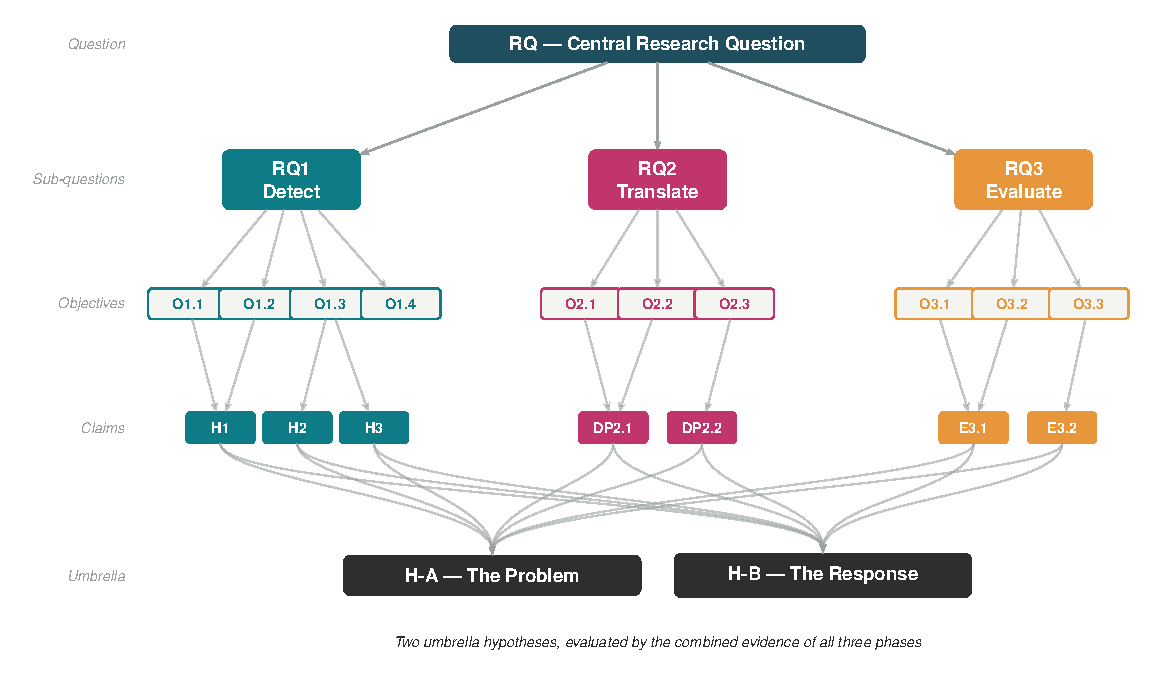
\includegraphics[width=\textwidth]{figures/research_questions/rq_tree_preview.pdf}
    \caption[Struttura delle domande di ricerca, degli obiettivi, delle affermazioni e delle ipotesi ombrello.]{\textbf{L'architettura
    del programma di ricerca.} La domanda di ricerca centrale si dirama in tre
    sotto-domande lungo l'arco rilevare--tradurre--valutare. Ogni sotto-domanda genera
    i propri obiettivi (O1.1--O1.4, O2.1--O2.3, O3.1--O3.3), che danno luogo alle
    affermazioni appropriate al loro carattere epistemico: ipotesi direzionali
    (H1--H3), proposizioni di design (DP2.1--DP2.2) e aspettative empiriche
    (E3.1--E3.2). Tutti e tre i gruppi di affermazioni convergono sulle due ipotesi
    ombrello, H-A (il problema) e H-B (la risposta), valutate non da un singolo
    strumento ma dall'evidenza combinata dell'intero programma.}
    \label{fig:rq-tree}
\end{figure}
